\chapter{Submanifolds}
\section{Basic definitions}

\begin{definition*}
    Let \(M\) be a topological manifolds. A subset \(S\subset M\) is a \dhighlight{topological submanifold},
    if \(S\) is a topological manifold with the subspace topology.
\end{definition*}

\begin{example}
    \(S^n=\{(x_0,\dots,x_n)\mid \sum x_i^2=1\}\subset\R^{1+n}\)
\end{example}
\begin{example}[Non-example]
    \(\{(x,y)\mid x=0\lor y=0\}\subset\R^2\), since this is not a manifold (see sheet 01).
\end{example}
\begin{definition*}
    Let \(M\) be a smooth manifold. A topological submanifold \(S\subset M\) is a \dhighlight{smooth submanifold}, if 
    it is equipped with a smooth structure, s.t. the embedding \(i:S\hookrightarrow M\) is smooth.   
\end{definition*}

\begin{example}
    If \(M\) is a smooth manifold and \(U\subset M\) open, then \(U\subset M\) is a smooth manifold.\marginnote{With the restricted smooth structure of \(M\)}
\end{example}

\begin{remark}
    Some authors (including Lee's textbook) use the term \dhighlight{embedded submanifold} to distinguish 
    from \dhighlight{immersed submanifolds}. For use ``submanifolds''\(\equiv\)``embedded submanifold''.
\end{remark}  

\begin{lemma}\label{lem:5.1}
    Suppose that \(f:M\to N\) smooth embedding. Let \(S\coloneqq F(M)\subset N\). Then 
    \(S\) admits a unique smooth structure making it a smooth submanifold, with the property that 
    \(f\) is a diffeomorphism onto its image.
\end{lemma}

\begin{proof}
    By definition of \(f\) being an embedding, \(f\) is a homeomorphism onto it's image, with the subspace topology.
    \(\implies S\) is a topological manifold. 

    We define a smooth atlas on \(S\) by taking \(\{(f(U),\varphi\circ f^{-1})\}\), as \((U,\varphi)\) ranges over the set of charts 
    for \(M\).

    Clearly \(f\) is a diffeomorphism, since \(\varphi\circ f\circ f^{-1}\circ\psi^{-1}\), for \((U,\varphi),(V,\psi)\) smooth charts, this follows 
    from the fact that \((U,\varphi),(V,\psi)\) are smoothly compatible on \(M\).

    This is the only smooth at with the property that \(f\) is a diffeomorphism, if \(\cB\) is an other such atlas, then the fact 
    that \(f\) is a diffeomorphism for \((S,\cB)\iff (S,\cA)\) compatible.

    Finally
    \begin{figure}[H]
        \centering
        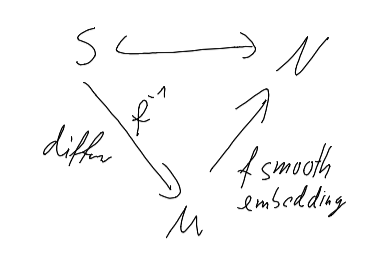
\includegraphics[width=.7\textwidth]{sketch_5_01.png}
        \caption{Sketch 5.01}
    \end{figure}
    so \(i\) is a smooth embedding.
\end{proof} 

\begin{definition*}
    A embedded submanifold \(S\) is called \dhighlight{properly embedded}, if the inclusion map 
    \(i\hookrightarrow N\) is proper (i.e. the preimage of a compact set is compact). 
\end{definition*}

\begin{example}
    \(S^n\hookrightarrow R^{n+1}\) properly embedded. 
\end{example}

\begin{example}[Non-example]
    \(S^n\setminus\{\text{pt}\}\subset\R^{n+1}\)
    \begin{figure}[H]
        \centering
        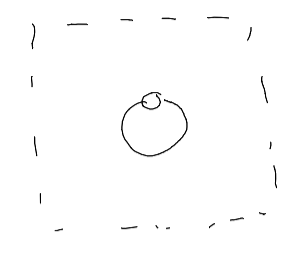
\includegraphics[width=.7\textwidth]{sketch_5_02.png}
        \caption{Sketch 5.02}
    \end{figure}
\end{example}

\begin{lemma}\label{lem:5.2}
    A topological submanifold \(S\subset N\) is properly embedded iff 
    \(S\) is closed.
\end{lemma}

\begin{proof}
    Exercise.\marginnote{Elementary exercise in point set topology}
\end{proof}

\section{The ``slice lemma''}

\begin{theorem}[Slice lemma\footnote{Lee \cite{smooth_manifolds} calls it a theorem}]\label{thm:5.3}
    \begin{enumerate}
        \item[(a)] Suppose \(S^k\subset M^n\) is a submanifold of codimension \(n-k\).\marginnote{this is also a definition of codimension: \(\dim M - \dim S\)}
                   Then, for all \(p\in S\), there exists a chart \((V,\psi),p\in U\subset N\), such that \[\psi(V\cap S)=\{(x_1,\dots,x_k,x_{k+1},\dots,x_n)\in \psi(V)\mid x_{k+1}=c_{k+1},\dots,x_{n}=c_n\}.\]  
        \begin{figure}[H]
            \centering
            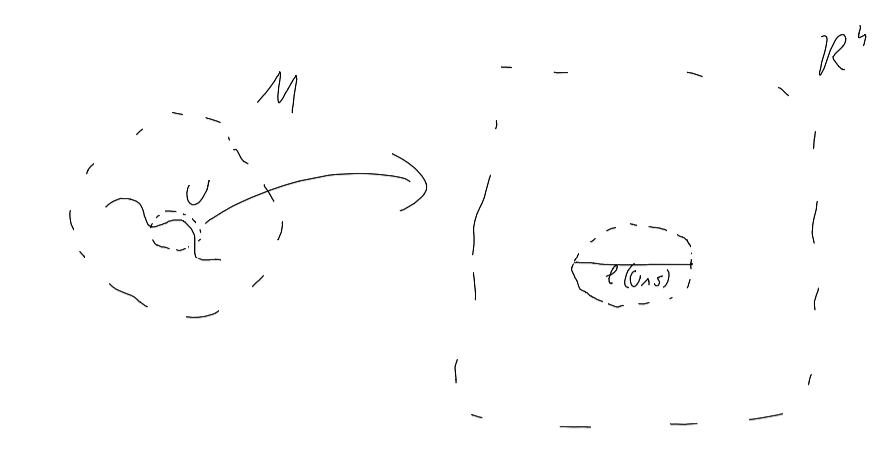
\includegraphics[width=.7\textwidth]{sketch_5_03.png}
            \caption{Sketch 5.03} 
        \end{figure}\markeol{09}\beginlecture{10}{12.11.2024}
        \item[(b)] Suppose that \(S\subset N\) is a subset with the property that, for all  \marginnote{The converse of (a)}
                   \(p\in S\), there exists a slice chart \((V,\psi),p\in V\subset N\), such that \[\psi(V\cap S)=\{(x_1,\dots,x_k,x_{k+1},\dots,x_n)\in \psi(V)\mid x_{k+1}=c_{k+1},\dots,x_{n}=c_n\},\]
                   then \(S\) admits a smooth manifold structure making it a smooth submanifold of \(N\).
    \end{enumerate}
\end{theorem}

\begin{remark}
    \begin{itemize}
        \item We get an equivalent theorem by requiring \(c_{k+1}=\dots=c_n=0\)
        \item Part (b) of theorem \ref{thm:5.3} tells us, that being a smooth submanifold \(S\subset N\) of ambient smooth manifold \(N\) is a property 
              property of the subset. It suffices to check, pointwise, the local property described above! 
    \end{itemize}
    % maybe different picture from phone?
\end{remark}

\begin{proof}
    \dhighlight{(a):} By assumption \(S\hookrightarrow N\) is an immersion. \marginnote{Locally, all immersions look the same}
    By theorem \ref{thm:4.3} (rank theorem), there exists charts \((U,\varphi),(V,\psi)\) such that \(i(U)\subset V\)
    and 
    \begin{align*}
        \hat{i}=\psi\circ i\circ \varphi^{-1}&:\varphi(U)\to\psi(V)\\
        (x_1,\dots,x_k)\mapsto (x_1,\dots,x_k,0,\dots,0)
    \end{align*}
    Up to shrinking \(\psi\) (restricting the image of \(\varphi\)), we find that 
    \[\psi(V\cap S)=\{(x_1,\dots,x_k,x_{k+1},\dots,x_n)\mid x_{k+1}=\dots=x_{n}=0\}\]
    \dhighlight{Warning:} What can go wrong here? Consider 
    \begin{figure}[H]
        \centering
        \includegraphics[width=.7\textwidth]{example-image}
        \caption{Sketch 5.04}
    \end{figure}
    Show that there is no more stuff in the set! % Will be fixed later

    \dhighlight{(b):} We have to check that the local charts given form an atlas. Which is almost a tautology and quite tedious, as we can use \(\{S\cap V,\psi\restrict{S}\}\) as the atlas.
\end{proof}

\begin{remark}[+Exercise]
    In section 2.1.2, example 4, we considered % todo: fix 
    \(\Phi:\R^{1+n}\to\R\). We assumed \(d\Phi\) is nonzero on 
    the set \(\Phi^{-1}(0)\subset\R^{1+n}\). Under this assumption, we proved 
    that \(\Phi^{-1}(0)\) is a naturally smooth manifold. Using theorem \ref{thm:5.3} (or by hand) 
    \(\Phi^{-1}(0)\) is a smooth submanifold.
\end{remark}

A priori, \(S\subset N\) could admit multiple smooth structures making it a submanifold. We know 
    seek to show that this is not the case.

\begin{lemma}\label{lem:5.4}
    Let \(S\subset N\) be a submanifold. If \(F:M\to N\) is a smooth map which factors through 
    \(S\hookrightarrow N\) as a continuous map, then \(F\) is smooth as a map \(M\to S\). 
    \begin{figure}[H]
        \centering
        \includegraphics[width=.7\textwidth]{example-image}
        \caption{Sketch 5.05}
    \end{figure}
\end{lemma}

\begin{proof} % TODO: Fix notation
    By theorem \ref{thm:5.3}, there exists \(U\subset S\hookrightarrow N\supset V\)
    \begin{figure}[H]\marginnote{More by the proof of the theorem ...}
        \centering
        \includegraphics[width=.7\textwidth]{example-image}
        \caption{Sketch 5.06}
    \end{figure}
Let us call \(\stackrel{\vee}{F}:M\to S,\stackrel{\vee}{F}(x)=F(x)\). Since \(\stackrel{\vee}{F}\) 
is continuous, \(\stackrel{\vee}{F^{-1}}(U)\subset M\) open. So, we can write, for \((W,u)\), \(W\subset \stackrel{\vee}{F^{-1}}(U)\)
\begin{figure}[H]
    \centering
    \includegraphics[width=.7\textwidth]{example-image}
    \caption{Sketch 5.07}
\end{figure}
were, a priori, \(\stackrel{\vee}{F^{i}}\) are continuous.

Concatenating the two diagrams, we find that \(F(x_1,\dots,x_m)=i\circ \stackrel{\vee}{F}(x_1,\dots,x_m)=(\stackrel{\vee}{F^1}(x_1,\dots,x_m),\dots,\stackrel{\vee}{F^k}(x_1,\dots,x_m),0,\dots,0)\).
But then each \(\stackrel{\vee}{F^i}\)  has to be smooth and therefore \(\stackrel{\vee}{F}\) is smooth.
\end{proof}

\begin{lemma}\label{lem:5.5}
    Let \(S\subset M\) be a subset satisfying the conditions of theorem \ref{thm:5.3} (b), then 
    the smooth structure produced by the theorem is the \dhighlight{unique} smooth structure, such that \(S \hookrightarrow M\) 
    is a smooth submanifold.
\end{lemma}

\begin{proof}%TODO: Fix
    Let \(\tilde{S}\) be a copy of \(S\), but endowed with some possibly different smooth structure s.t. \(\tilde{S}\hookrightarrow M\) 
    is an embedding.\marginnote{Ergo it is a smooth submanifold of \(M\)}
    
    \(\tilde{S}\hookrightarrow M\) factors through \(S\), so \(\tilde{S}\stackrel{\text{id}}{\to} S\) smooth. Similarly \(S\stackrel{\text{id}}{\to} \tilde{S}\) smooth.\marginnote{This uses lemma \ref{lem:5.4}}
\end{proof}

\section{The (weak) Whitney embedding theorem}

\begin{theorem}[Whitney]\label{thm:5.6:whithney}
    Every compact \(n\)-dimensional smooth manifold admits an embedding into \(\R^N\) for 
    \(N\gg 1\) large enough.
\end{theorem}

\begin{remark}
    Later (probably this month), we will remove the compactness assumption and also argue that one 
    can take \(N=2n+1\).

    Whitney proofed that one can take \(N=2n\).\marginnote{Don't sue him, if he is off by one :)}
\end{remark}

\begin{aremark}
This is a very philosophically pleasing statement, since we recover our intuition of embedded manifold from the abstract theory. It is also true, that there is only one embedding (up to isotopy). 
\end{aremark}

\begin{proof}[Proof of theorem \ref{thm:5.6:whithney}]
    Fix a finite cover of \(M\) \(\{B_1,\dots,B_k\},B_i\subset M\) open. We may as well assume 
    that there exist charts \((B_i',\phi_i),\overline{B_i}\subset B_i',\varphi_i(B_i')=B_1(0)\subset \R^m\).

    Let \(\rho_i:M\to \R\) be a cutoff function for \((\overline{B}_i\subset B_i')\), i.e. \(\rho_{i\mid_{B_i}}=\equiv 1,\supp (\rho_i)\subset B_i',0\leq \rho_i\leq 1\).
    The existence of the \(\rho_i\) follows from proposition \ref{prop:2.8}. 

    We now define \marginnote{Notice the \(k\) comes from compactness, i.e. we have no control over it, as it its non-constructive}
    \begin{align*}
        F:M&\to \R^{mk+k}\\
        p&\mapsto (\rho_1(p)\underbrace{\varphi_1(p)}_{\in \R^m},\dots,\rho_k(p)\varphi_k(p),\rho_1(p),\dots,\rho_k(p))
    \end{align*}
    We will now see that \(F\) is an embedding. First, we will argue \(F\) is an injective immersion.

    If \(F(p)=F(q)\implies \rho_i(p)=\rho_i(q)\forall i=1,\dots,k\). Let \(i_0\) be such that \(p\in B_{i_0}\). Then 
    \(\rho_{i_0}(p)=1=\rho_{i_0}(q)\implies\) \(q\in \supp(\rho_{i_0})\subset B_{i_0}'\). But 
    now \(\underbrace{\varphi_{i_0}(p)}_{\in\R^m} = \rho_{i_0}(p)\varphi_{i_0}(p)=\rho_{i_0}(q)\varphi_{i_0}(q)=\varphi_{i_0}(q)\). Hence \(p,q\in B_{i_0}'\implies p=q\).

    \dhighlight{\(F\) is an immersion:} Choose \(p\in M\). Then p \(p\in B_{i_0}\), for some 
    \(i_0\). Hence \(\rho_{i_0}\equiv 1\) for some neighborhood of \(p\).
    \begin{figure}[H]
        \centering
        \includegraphics[width=.7\textwidth]{example-image}
        \caption{Sketch 5.08}
    \end{figure}
    Hence \(d(\rho_{i_0}\varphi_{i_0})=\underbrace{d\rho_{i_0}}_{\text{ invertible }m\times m}\) near \(p\implies dF\) is injective near \(p\), but \(p\) was arbitrary.

    Finally,\marginnote{Kind of cheating ...}
    since \(M\) is compact, the theorem follows from the following lemma \ref{lem:5.7}.

    I.e. it is enough to show that \(F^{-1}:F(M)\to M\) is continuous, i.e. 
    \(F:M\to F(M)\) is a closed map. But since \(M\) is compact, \(F\) is proper \(\stackrel{\text{lemma \ref{lem:5.7}}}{\implies} F\) closed.

\end{proof}


\begin{lemma}[Lee Appendix A: 57]\label{lem:5.7}
    Let \(X\) be a topological space. Let \(Y\) be locally compact (e.g. a topological manifold),
    then any proper continuous map % TODO: proper ... 
    is closed.
\end{lemma}